\chapter{Analisis dan Perancangan}
\label{chap:analisisdanperancangan_hasilStudi}

\section{Analisis Masalah dan Solusi}
\label{sec:analisisdanperancangan_masalahdansolusi}
Pada bagian ini, dilakukan analisis terhadap masalah propagasi \textit{workflow} dengan sistem email. Analisis ini akan menjawab \textit{event} yang terkait dengan integrasi sistem email dan mekanisme integrasi BPMS dan sistem email.

\subsection{Analisis Masalah}
\label{analisisdanperancangan_analisismasalah}
Pada bab sebelumnya, telah dijelaskan langkah-langkah untuk mengotomasi proses bisnis menggunakan BPMS Camunda. Dalam proses otomasi tersebut, ada beberapa hal yang dibutuhkan agar proses otomasi berjalan dengan lancar. Untuk mengidentifikasi hal-hal yang dibutuhkan tersebut, berikut adalah \textit{workflow} yang menjelaskan langkah-langkah mengotomasi proses bisnis menggunakan BPMS Camunda :

		\begin{figure}[H]
			\centering
			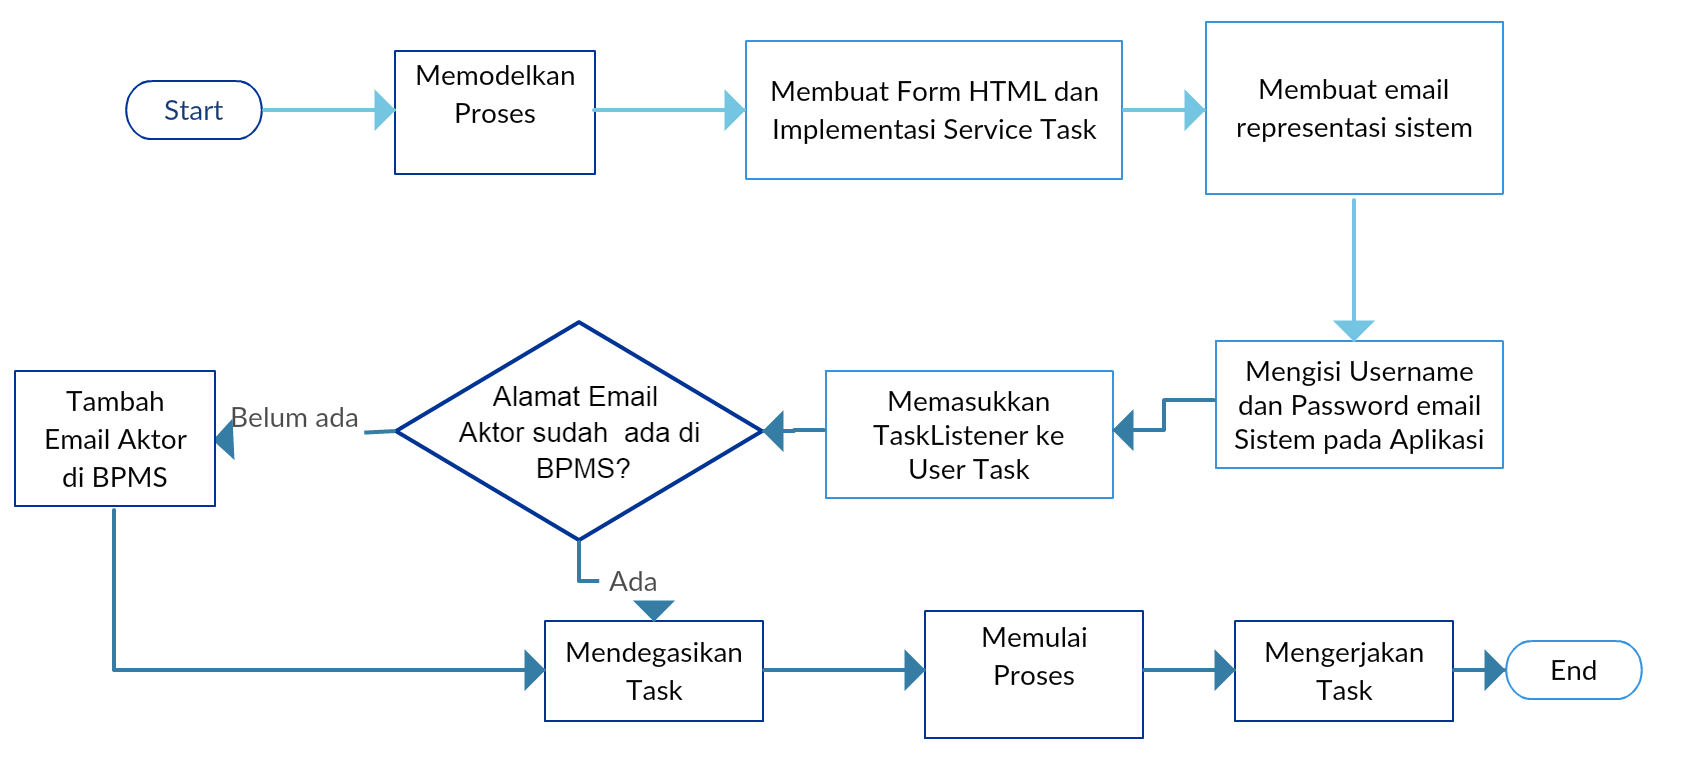
\includegraphics[scale=0.4]{Gambar/Bab-4/HighLevelFlowchart}
			\caption{Flowchart Otomasi Proses Bisnis} 
			\label{fig:stepflowchart}
		\end{figure}

Berdasarkan \textit{flowchart} ini, maka untuk mempropagasi email ada beberapa hal yang dibutuhkan, yaitu :
\begin{enumerate}
	\item Model proses menggunakan BPMN yang sudah dilengkapi form HTML untuk \textit{user task}, implementasi untuk \textit{service task} dan atribut lain yang diperlukan.
	\item Alamat email yang merepresentasikan sistem.
	\item Algoritma untuk mengirim email (TaskListener).
	\item Kumpulan \textit{user/group} yang akan mengerjakan \textit{task}.
	\item Business Process Management System (BPMS), yaitu tools untuk mengotomasi jalannya proses.
\end{enumerate}


Kebutuhan tersebut dibagikan ke tiga partisipan yang memiliki perannya masing-masing, yaitu desainer, admin, dan aktor.

\begin{enumerate}
\item Tugas Desainer 
Seorang desainer model proses memiliki beberapa tugas, yaitu :
\begin{enumerate}
	\item Merancang model proses.
	\item Menambahkan form HTML pada \textit{user task}, \textit{implementasi service task}, \textit{task listener} untuk propagasi email, dan berbagai atribut lainnnya sesuai kebutuhan.
	\item Membuat alamat email yang merepresentasikan sistem.
	\item Menambahkan \textit{username}, \textit{password}, dan \textit{host} email pada aplikasi task listener.
	\item Mendelegasikan task kepada user/group yang akan mengerjakan.
\end{enumerate}

\item Tugas Admin
Seorang admin memiliki dua tugas, yaitu :
\begin{enumerate}
	\item Menambahkan user/group yang akan mengerjakan \textit{tasks} pada Camunda Admin.
	\item Menjalankan dan memulai proses.
\end{enumerate}

\item Tugas Aktor
Seorang aktor memiliki dua tugas, yaitu :
\begin{enumerate}
	\item Memberitahu alamat email kepada admin.
	\item Mengerjakan \textit{task}.
\end{enumerate}

\end{enumerate}


\subsection{Usulan Solusi}
\label{sec:usulansolusi}

\begin{enumerate}
\item\textit{Event} yang Terkait dengan Integrasi Sistem Email
\label{sec:eventUserTask}

Integrasi Camunda dengan sistem email pada skripsi ini bertujuan untuk memberi tahu aktor Camunda apabila ada \textit{tasks} yang perlu dikerjakan oleh aktor. Ketika aktor menerima email mengenai \textit{tasks} yang perlu dikejakan, aktor dapat langsung mengerjakannya. 

Camunda memiliki berbagai jenis \textit{tasks} seperti \textit{user tasks, manual tasks, service task}, dan lainnya. Karena proses integrasi email dengan Camunda melibatkan aktor (aktor menerima pemberitahuan pekerjaannya melalui email), \textit{task} yang akan diintegrasikan dengan sistem email adalah \textit{user tasks}.

\item Mekanisme Integrasi Sistem Email
\label{integrasi}
\textit{User tasks} memiliki atribut \textit{Task Listener} yang dapat mengeksekusi perintah. \textit{Task Listener} memiliki dua atribut, yaitu \textit{Event Type} dan \textit{Listener Type}. Terdapat empat pilihan dari \textit{Event Type}, yaitu \textit{create, assignment, complete, delete}. 
		\begin{figure}[H]
			\centering
			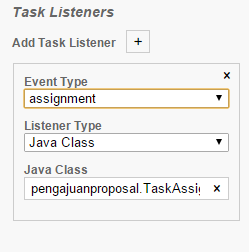
\includegraphics[scale=1]{Gambar/Bab-3/TaskListener}
			\caption{Event Task Listener} 
			\label{fig:eventtasklistener}
		\end{figure}
\begin{itemize}
	\item Create, perintah dieksekusi ketika \textit{task} telah dibuat dan siap untuk dikerjakan. 
	\item Assignment, perintah dieksekusi ketika aktor yang akan mengerjakan \textit{task} sudah ditentukan.
	\item Complete, perintah dieksekusi ketika \textit{task} sudah dikerjakan dan sebelum \textit{task} dihapus.
	\item Delete, perintah dieksekusi setelah \textit{task} dihapus.
\end{itemize}


Untuk mengintegrasikan \textit{user tasks} dengan email, \textit{event type} yang dapat digunakan adalah \textit{create} dan \textit{assignment}. \textit{Event complete} dan \textit{delete} tidak dapat digunakan untuk memberi tahu aktor karena setelah \textit{task} selesai dan dihapus, alamat email untuk \textit{Task} selanjutnya belum diambil sementara \textit{event} sudah selesai dipanggil.

Apabila menggunakan \textit{event create}, \textit{task} harus memiliki pemiliknya masing-masing ketika BPMN dibuat atau memiliki \textit{candidate user/group}. Bila pemilik \textit{task} belum ditentukan, email tidak akan terkirim, karena \textit{event create} sudah selesai dipanggil sebelum \textit{task} memiliki pemilik. Pengiriman email untuk \textit{task} yang belum memiliki aktor dapat menggunakan \textit{event create}. Sedangkan pada \textit{event assignment}, pengiriman email dilakukan setelah \textit{task} didelegasikan ke masing-masing user.


\end{enumerate}


\section{Rancangan Sistem}
\label{sec:analisisdanperancangan_rancangansistem}
Untuk mengimplementasikan integrasi email dengan sistem BPMS, ada beberapa hal yang perlu dirancang terlebih dahulu, seperti rancangan email yang akan dikirim, algoritma untuk pengiriman email, dan rancangan antarmuka.

\subsection{Rancangan Email}
\label{Rancangansistem_rancanganemail}
Alamat email yang digunakan untuk merepresentasikan sistem berbasis Gmail SMTP. Server Gmail SMTP memiliki batas pengiriman email sebanyak 2.000 email per hari. Gmail SMTP yang akan digunakan memiliki konfigurasi sebagai berikut \cite{smtpgoogle} :
\begin{itemize}
	\item Alamat server = smtp.gmail.com.
	\item Port = 587 (menggunakan TLS).
	\item Username Gmail.
	\item Password Gmail.
\end{itemize}
Email yang akan dikirimkan ke aktor memiliki format :
\begin{enumerate}
	\item Subjek.
	\item Nama aktor.
	\item Nama \textit{task}.
	\item Tautan ke \textit{task}, yaitu http://localhost/camunda/app/tasklist/default/\#/?task=(\textit{id task}).
\end{enumerate}
Berikut adalah contoh email yang akan dikirim :
			\begin{figure}[H]
			\centering
			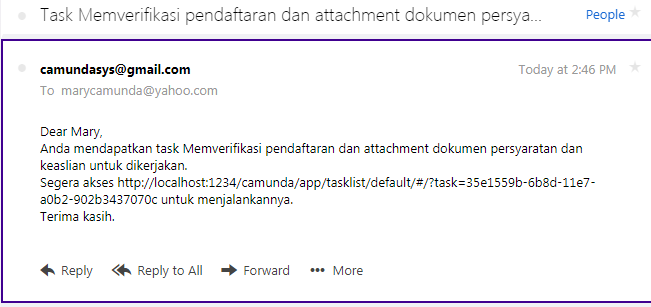
\includegraphics[scale=0.8]{Gambar/Bab-5/kasus2/12}
			\caption{Contoh Email} 
			\label{fig:perancangan_contohemail}
	\end{figure}
 

\subsection{Rancangan Algoritma Pengiriman Email}
\label{sec:Rancangansistem_algoritma}
\begin{itemize}

\item Untuk mengirim email ke pemilik \textit{task}, langkah-langkahnya adalah sebagai berikut :
\begin{enumerate}
	\item Mengambil id dari \textit{task}.
	\item Mengambil informasi aktor yang akan mengerjakan \textit{task}. Informasi aktor yang mengerjakan task didapatkan dari kolom assignee, candidateUser, atau candidateGroup.
	\item Jika assignee memiliki nilai, email dikirim ke aktor pada kolom assignee, jika tidak maka email dikirim ke aktor pada kolom candidateUser dan/atau CandidateGroup. 
	\item Membangkitkan subjek dan isi email yang berisi tautan ke \textit{task} yang akan dikerjakan. 
	\item Membuat koneksi ke email server dengan \textit{username} dan \textit{password}
	\item Mengirim email.
\end{enumerate}

Berikut adalah pseudocode untuk mengirim email ke pemilik \textit{task} :

\begin{lstlisting}[basicstyle=\tiny,caption=Pseudocode TaskAssignmentListener]
taskListener(){
	Mengambil nilai assignee 
	Mengambil taskId
	Mengambil taskName
	Mengambil candidateUsers
	Mengambil candidateGroup
	Mengambil username Gmail
	Mengambil password Gmail
	
	IF assignee punya nilai Then
		sendEmail(user)
	ELSE
		IF candidateUser punya nilai THEN
			sendEmail(candidateUser)
		ENDIF
		IF candidateGroup punya nilai Then
			FOR setiap user di candidateGroup
				sendEmail(user)
			ENDFOR
		ENDIF
	ENDIF
}

sendEmail(user){
	Menentukan port menjadi 587
	Menentukan status auth menjadi true
	Menentukan status tls menjadi true
	
	Membuat koneksi ke server dengan username dan password Gmail untuk autentikasi
	
	Menentukan penerima email dari user
	Menentukan subjek email yaitu ("Task" + taskName)
	Menentukan isi email yaitu ("Dear " + user.getName() + \n + "Anda mendapatkan task " +taskName +" untuk dikerjakan \n Segera akses http://localhost:1234/camunda/app/tasklist/default/#/?task="+taskId +"untuk menjalankannya. \n Terima kasih.")

	Mengirim email
}

\end{lstlisting}

%\subsection{\textit{Task Event Listener}}
%\label{sec:perancangansistem_taskeventlistener}
\item \textit{Task Event Listener} bereaksi ke \textit{Task Event} seperti \textit{Created, Assigned, dan Completed}. Implementasi \textit{Task Listener} berupa kode Java dapat dilihat di bawah ini :
\begin{lstlisting}[language=Java,basicstyle=\tiny,caption=TaskAssignmentListener.java]
public class TaskAssignmentListener implements TaskListener{
	public void notify(DelegateTask delegateTask) {
	
	}
}
\end{lstlisting}

Parameter delegateTask dapat mengambil maupun menyimpan informasi \textit{task} yang sedang berjalan. Beberapa informasi yang dapat diambil maupun disimpan adalah sebagai berikut :
\begin{itemize}
	\item getAssignee(), mendapatkan pemilik \textit{task} dan setAssignee untuk menentukan pemilik \textit{task}
	\item getId(), mendapatkan id dari \textit{task}
	\item getName(), mendapatkan nama \textit{task} dan setName untuk menentukan nama\textit{task}
	\item getCandidates(), mendapatkan \textit{candidate users/groups} dan addCandidateGroup() / addCandidateUser() untuk menentukan \textit{candidate users/groups}
	
\end{itemize}
\end{itemize}

\subsection{Rancangan Antarmuka untuk Membangkitkan Kode \textit{Task Event Listener}}
\label{sec:perancangansistem_antarmuka}
Antarmuka yang digunakan memiliki dua masukan, yaitu email dan password Gmail yang merepresentasikan sistem. Ada dua tombol, yaitu tombol untuk memilih direktori tujuan dan tombol untuk membangkitkan kelas Java yang berisi \textit{Task Event Listener} pada direktori yang telah dipilih sebelumnya. Berikut adalah tampilan antarmukanya :

	\begin{figure}[H]
			\centering
			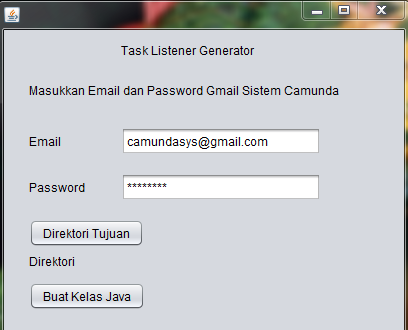
\includegraphics[scale=1]{Gambar/Bab-4/UI/1}
			\caption{Tampilan Antarmuka untuk Membangkitkan Kode \textit{Task Event Listener}} 
			\label{fig:perancangansistem_antarmuka}
	\end{figure}
	


 